
%
%  $Description: Author guidelines and sample document in LaTeX 2.09$ 
%
%  $Author: ienne $
%  $Date: 1995/09/15 15:20:59 $
%  $Revision: 1.4 $
%

\documentclass[times, 10pt,twocolumn]{article} 
\usepackage{latex8}
\usepackage{times}
\usepackage[ngerman]{babel}
\usepackage[utf8]{inputenc}
\usepackage{color}
\usepackage{graphicx}
\usepackage{capt-of}
\usepackage{amsmath}
\usepackage{amsfonts}



%\documentstyle[times,art10,twocolumn,latex8]{article}

%------------------------------------------------------------------------- 
% take the % away on next line to produce the final camera-ready version 
\pagenumbering{arabic}

%------------------------------------------------------------------------- 
\begin{document}

\title{Distributed Computation of Disparity Maps on multiple GPUs using TCP sockets}

\author{Eric Buschermöhle, Sven Frank, Timo Janssen\\
Technische Universität Braunschweig \\  38106 Braunschweig, Deutschland\\
e.buschermoehle@tu-bs.de\\
sven.frank90@gmail.com\\
timo-janssen@kabelmail.de\\
}


\maketitle
\thispagestyle{empty}

\begin{abstract}
Die Verlagerung von parallelisierbaren Berechnungen von der CPU auf die Grafikkarte eines Rechners ermöglicht eine deutliche Steigerung der Rechengeschwindigkeit. Die CUDA-Plattform von NVIDIA erweitert die Sprache C um Elemente zur parallelen Programmierung für geeignete Grafikkarten des Unternehmens. Eine weitere Steigerung der Rechenleistung lässt sich durch den Einsatz mehrerer Grafikkarten erreichen. Da normale Rechner in der Regel nur über eine Grafikkarte verfügen, bietet sich die Verteilung des Problems über ein Netzwerk auf mehrere Rechner an. In dieser Arbeit wird am Beispiel einer Disparitätenberechnung von Stereobildern die Implementierung eines vorhandenen Algorithmus auf der GPU und die Aufteilung auf mehrere vernetze Computer beschrieben und evaluiert.
 
\end{abstract}



%------------------------------------------------------------------------- 
\Section{Einführung}

Zum Auffinden von korrespondierenden Punkten in einem Stereobildpaar werden verschiedene Stereoanalyseverfahren eingesetzt. Mit Hilfe der gefundenen Korrespondenzen und den intrinsischen sowie extrinsischen Parameter des Stereokamerasystems ist es möglich durch Triangulation eine Szene 3D rekonstruieren. Stereoanalyseverfahren finden ihren Einsatz im industriellen Umfeld unter anderem im Bereich der Qualitätssicherung. Aber auch Anwendungsfelder in der Robotik und Automobilindustrie, zum Beispiel zur Hinderniserkennung, sind potentielle Anwendungsbereiche. Neben einer möglichst dichten und genauen Tiefenkarte spielen Laufzeitaspekte eine entscheidende Rolle. In dieser Arbeit wird das Laufzeitverhalten anhand einer Korrelationsmethode exemplarisch untersucht. Es werden insgesamt zwei Möglichkeiten zur Beschleunigung des Verfahrens vorgestellt. In einem ersten Schritt erfolgt die Parallelisierung auf der GPU (Graphics Processing Unit) mit der von Nvidia entwickelten Programmier-Technik CUDA. In einem zweiten Schritt erfolgt die Verteilung der Anwendung auf über ein Netzwerk verbundene Rechner. Zu diesem Zweck werden TCP-Sockets eingesetzt.

%------------------------------------------------------------------------- 
\SubSection{Korrelationsmethode}

Der Algorithmus benötigt ein Referenzbild sowie ein Suchbild, welche beide entzerrt und rektifiziert sein müssen. Die Vorgehensweise zur Bestimmung der Disparität ist dabei wie folgt: Ausgehend von einem Bildpunkt $(u_1,v_1)$ im Referenzbild wird ein Referenzfenster der Größe \textit{MaskWidth} und \textit{MaskHeight} um den Ausgangspunkt gewählt und mit entsprechenden verschobenen Suchfenstern aus dem Suchbild entlang einer korrespondierenden Zeile (Epipolarlinie) verglichen. Dies entspricht also der Bestimmung der Ähnlichkeit zweier gleichgroßer Fenster. Unter Verwendung einer Kostenfunktion kann die Bildposition $(u2, v2)$ ermittelt werden, die für das gewählte Referenzfenster im Referenzbild das ähnlichste Suchfenster im Suchbild darstellt d.h. die niedrigsten Kosten besitzt. Die Differenz der Punkte $(u_1,v_1)$ und $(u_2,v_2)$ wird Disparität $d(u_1,v_1)$ genannt und wird zur Bestimmung der Tiefe einer Szene benötigt. Weiterführende Literatur ist in \cite{Hartley.2003} und \cite{Schreer.2005} zu finden. Wurden für alle Bildpunkte in einem Bild die Disparitäten gefunden, werden diese zu einer sogenannten Disparitätskarte oder auch Tiefenkarte zusammengefügt. In Abbildung \ref{fig:korrelationsmethoden} ist ein Referenzfenster und ein um die Disparität $d(u,v)$ verschobenes Suchfenster dargestellt.

\begin{figure}[!ht]
	\centering
	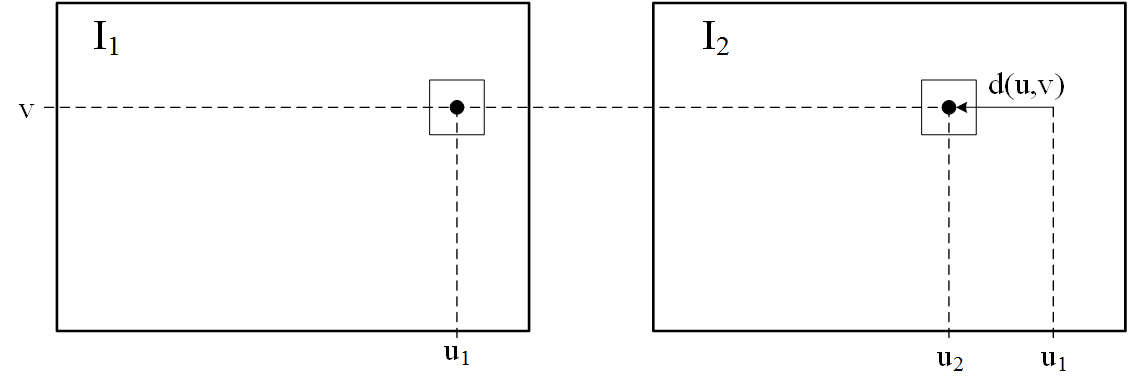
\includegraphics[width=0.9\linewidth]{image/korrelationsverfahren.png}
	\captionof{figure}[Korrelationsmethoden]{Darstellung der Fenster in beiden Bildern zur Bestimmung der Ähnlichkeit}
	\label{fig:korrelationsmethoden}
\end{figure}

%------------------------------------------------------------------------- 
\SubSection{Kostenfunktion}

Als Kostenfunktion wird in dieser Arbeit der mittlere absolute Fehler (engl. sum of absolute differences (SAD)) eingesetzt. Mit diesem wird die absolute Differenz zwischen zwei Fenstern berechnet. Die Ähnlichkeit ist dort am größten, wo die Differenz minimal wird:

\begin{align}
\small 
\begin{split}
C(u,v,d) = \frac{1}{N}\sum\limits_{m} \sum\limits_{n} | g_1(u+m,v+n) - \\ g_2(u+d(u,v)+m,v+n)|
\label{eq:sad}
\end{split}
\end{align}

%------------------------------------------------------------------------- 
\Section{Related Work}

Die Berechnung von Tiefenkarten auf der GPU ist nicht neu. In der Arbeit von \cite{Yang.2002} wird eine Methode vorgestellt, die Korrelationsmethoden basierend auf der Kostenfunktion SAD mit Hilfe der GPU berechnet. In \cite{Woetzel.2004} erfolgt die Berechnung der Tiefenkarte mit der Kostenfunktion SSD (engl. sum of absolute differences). Die Bildvorverarbeitung und Nachbereitung erfolgt dabei ebenfalls auf der GPU. Als Ergebnis konnte eine Beschleunigung der Verarbeitungsgeschwindigkeit auf 20fps erreicht werden.

Aktuellere Arbeiten beschäftigen sich mit der Beschleunigung des von Hirschmüllers vorgestellten Semi-Global Matching (SGM) \cite{Hirschmuller.2005} zum Erzeugen von Tiefenkarten. Ein Beispiel dafür ist die Arbeit \cite{Hirschmueller.2008} und \cite{Rosenberg.2006}, in welchen die Berechnung von Tiefenkarten mit dem SGM und CUDA implementiert wurden.

%------------------------------------------------------------------------- 
\Section{Konzept}
\paragraph{Graphics Processing Unit}
Der Grafikprozessor ist ein auf Berechnung von Grafiken spezialisierter und optimierter Prozessor in einem Computer oder einem anderen Gerät mit visueller Ausgabe.
Der Cache-Speicher der GPU (Graphic Processing Unit) ist im Gegensatz zur CPU erheblich kleiner dimensioniert. Zudem existiert kein Raum für komplexe Logik. Grundsätzlich ist die Recheneinheit der Grafikkarte so aufgebaut, dass möglichst viele eher einfache Rechenoperationen parallel möglich sind.
Diese Algorithmic Logic Units (ALU) sind wie in Abbildung \ref{fig:gpu} dargestellt in wesentlich höhrerer Anzahl auf der GPU vorhanden. Sie lassen sich wiederum jeweils in eine bestimmte Anzahl an Blöcke unterteilen, wobei jeder Block selbst mehrere Threads aufrufen kann. Durch diese Unterteilung ermöglicht der Grafikprozessor eine wesentlich schnellere Berechnung von einfachen arithmetischen Aufgaben.

 \begin{figure}[!ht]
	\centering
	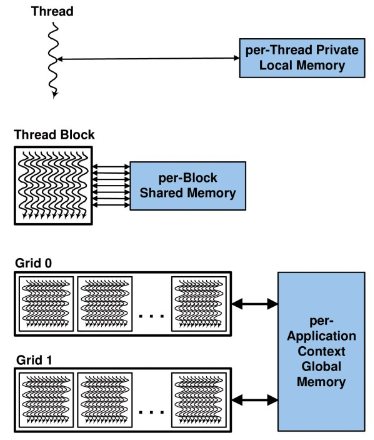
\includegraphics[width=0.9\linewidth]{image/cuda.jpg}
	\captionof{figure}[Ansatz]{Aufbau von CPU und GPU im Vergleich \cite{CUDA.2015}}
	\label{fig:gpu}
\end{figure}

\paragraph{Idee}
In dieser Arbeit geht es zunächst darum die Berechnung der Tiefenkarte von der CPU auf die GPU auszulagern. Dazu wird eine entsprechende Programmiertechnik verwendet werden, um die notwendigen Daten auf den Grafikspeicher zu transferieren. In einem zweiten Schritt erfolgt die Optimierung der Berechnung durch massive Parallelisierung zur Laufzeitreduzierung auf der GPU. 

Als weitere Möglichkeit zur Reduzierung der Laufzeit, wird eine Client-Sever Anwendung entwickelt. Durch diesen Sachverhalt ist die Aufteilung der Anwendung auf verschiedene Clients im Netzwerk möglich. Ziel ist es, die Berechnungen auf dem jeweiligen Client ebenfalls auf der GPU zu parallelisieren. Das Gesamtkonzept kann wie folgt zusammengefasst werden: In einem ersten Schritt erfolgt die Segmentierung des Bildes entlang einer Bildzeile. Die Segmente werden anschließend über das Netzwerk an die Clients verteilt. Im Anschluss führt jeder Client auf seiner GPU eine Berechnung der Tiefenkarte für seine Segmente durch. Abschließend sollen die berechneten Tiefenkarten an den Server gesendet werden, welcher diese zu einer gesamten Tiefenkarte zusammenfügt. 

%------------------------------------------------------------------------- 
\Section{Implementierung}
\SubSection{Optimierung von CPU auf GPU}

CUDA (Compute Unified Device Architecture) ist eine vom Grafikkarten-Hersteller Nvidia entwickelte Programmiertechnik, welche die Durchführung von einfachen Berechnungen auf der GPU erlaubt. Im Folgenden soll der Aufbau kurz erläutert werden.
  
 \begin{figure}[!ht]
	\centering
	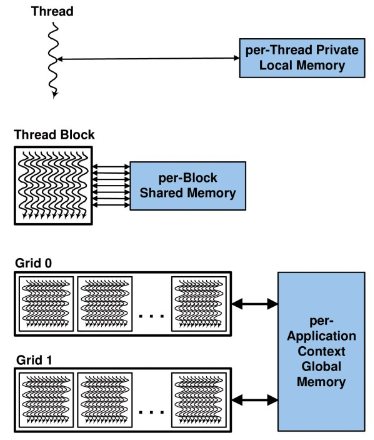
\includegraphics[width=0.7\linewidth]{image/cuda.png}
	\captionof{figure}[Aufbau CUDA]{Thread-Hierarchie und Speicherverwaltung von CUDA \cite{CUDA.2015}}
	\label{fig:cudaAufbau}
\end{figure}

Im Zusammenhang mit CUDA stellt der Begriff Kernel eine zentrale Rolle dar. Ein Kernel wird von einer Vielzahl hierarchisch angeordneter Threads auf der GPU ausgeführt. Jeder dieser Threads besitzt seinen eigenen privaten Speicherbreich (per-Thread Private Local Memory). Im Fall von CUDA C handelt es sich um eine in C geschriebene Funktion. Die einzelnen Threads werden in mehrdimensionalen Threadblöcken organisiert und erhalten eindeutige IDs. Alle Threads innerhalb eines Blocks teilen sich einen gemeinsamen Speicher (Per-Block Shared Memory) auf welchen der Zugriff synchronisiert erfolgen muss. Die verschiedenen Blöcke werden wiederum in sogenannte Grids  organisiert, die ebenfalls eine eindeutige ID erhalten. Jedes Grid stellt dabei ein eigenständiges Kernel dar. Abbildung \ref{fig:cudaAufbau} veranschaulicht diesen Aufbau. (Vgl. \cite{CUDA.2015})

Praktisch ergibt sich dann folgender Aufbau: der Entwickler schreibt einen Kernel, welcher die Programmlogik enthält die auf der GPU ausgeführt werden soll. Darüber hinaus muss der Host-Code geschrieben werden, welcher das eigentliche Programm in der jeweiligen Programmiersprache enthält. Dieser führt den Transfer von benötigten Daten auf den Grafikspeicher aus und ruft anschließend den Kernel auf. Nach Durchführung des Kernels müssen die berechneten Daten wieder von der GPU auf die CPU kopiert werden um dort eine Weiterverarbeitung realisieren zu können.

Eine Parallelisierung ist hierbei durch den Entwickler möglich. Dieser kann durch von CUDA bereitgestellte Funktionen steuern, auf wie viele Blöcke und Threads der entsprechende Kernel aufgeteilt werden soll.

\paragraph{Entwicklung und Paralellisierung des Kernels}
Der Kernel wurde aus der bereits vorhandenen iterativen Implementierung des Algorithmus entwickelt. Da die Berechnung der Disparität der einzelnen Bildpunkte unabhängig voneinander erfolgt, ist es naheliegend, diese zu parallelisieren. Hierzu wurden die beiden äußersten Schleifen, die für die Iteration über die einzelnen Bildpunkte zuständig sind, entfernt.  
Aufgrund der limitierten Anzahl an Threads pro Block ist eine Aufteilung der Pixel einer Zeile auf einen Block nicht sinnvoll. Übersteigt die Pixelzahl pro Zeile die Limitierung, treten Fehler auf. Stattdessen wird eine feste quadratische Blockgröße gewählt. Die Größe des Grids wird aus der Blockgröße und der Anzahl an Zeilen und Spalten des Bildes berechnet und aufgerundet, damit alle Bildpunkte abgedeckt werden. Im Kernel selbst kann über die \textit{BlockID}, die Blockgröße und die \textit{ThreadID} bestimmt werden, für welchen Bildpunkt der Thread ausgeführt wird. Um Fehler bei den am äußersten Rand gelegenen Blöcken zu vermeiden, wird im Kernel abgefragt, ob der Thread noch einem Bildpunkt zugeordnet ist oder dieser außerhalb des Bildes liegt.
Bis auf die aufgrund der syntaxspezifischen Unterschiede notwendigen Änderungen waren keine weiteren Anpassungen des Algorithmus an die parallele Verarbeitung notwendig.

\SubSection{Parallelisierung über TCP/IP}

\paragraph{Netzwerkkommunikation}
Bei Sockets handelt es sich um ein vom Betriebssytem bereitgestelltes Objekt, welche als Kommunikationsendpunkte betrachtet werden können. Durch diese Socktes können Daten empfangen und versendet werden, wobei verschiedene Techniken zur Übermittlung auf der Transportschicht verwendet werden können.
Ein bekanntes und im Zuge dieser Arbeit verwendetes Modell nutzt TCP/IP zur Kommunikation (vgl. Abbildung \ref{fig:tcpip}). Dabei sorgt das Transmission Control Protocol für eine zuverlässige Übertragung der Daten auf Basis vom Internet Protocol (IP). Die Übermittlung der Pakete ist dabei garantiert. Sollte ein Fehler auftreten, so erhält der Sender eine Fehlermeldung und kann die Daten erneut senden. Grundsätzlich entspricht die Reihenfolge der eingehenden Pakete der Sendereihenfolge.
Die Verbindung zwischen zwei Kommunikationspartnern wird bei diesem Mechanismus durch die IP-Adressen und eine gemeinsame Portnummer hergestellt.\cite{Willemer.2007}

 \begin{figure}[!ht]
	\centering
	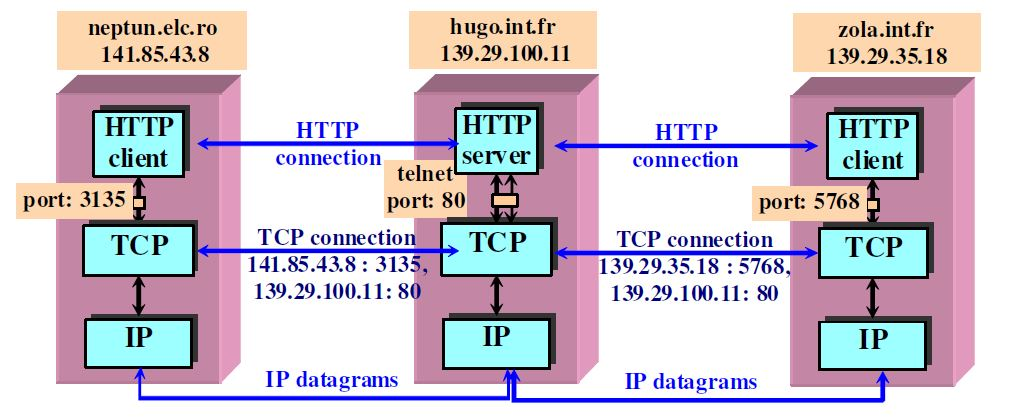
\includegraphics[width=0.9\linewidth]{image/ip-tcp.jpg}
	\captionof{figure}[Parallelisierung]{Kommunikationschema von TCP/IP \cite{Werner.2015}}
	\label{fig:tcpip}
\end{figure}

\paragraph{Client-Server Anwendung}
Die Berechnung der Disparität kann für horizontale Bildabschnitte unabhängig voneinander erfolgen und lässt sich daher auf mehrere Server verteilen. Zu beachten ist hierbei der obere und untere Randbereich der einzelnen Bildabschnitte, der für die Höhe der verwendeten Bildmatrix ausreichend groß sein muss, da andernfalls die am Rand gelegenen Zeilen nicht ausgewertet werden.

Die Serveranwendung wird an einem Port gebunden und wartet auf eine Verbindungsanfrage. Wird eine Verbindung hergestellt, erwartet die Anwendung zunächst die Metadaten der zu bearbeitenden Bilder. Neben den Informationen zur Bildgröße werden hierbei auch die Parameter der Berechnung übertragen. Anschließend wird zunächst das linke, dann das rechte Bild übertragen, wobei die Bildgröße anhand der Metadaten überprüft wird. Da die Übertragung der Daten binär erfolgt, entsteht deutlich weniger Overhead als bei einer Implementierung mit einem SOAP-basiertem Webservice. Die Disparität wird auf der GPU des Servers berechnet und an den Client zurückgesendet. Dieser fügt die einzelnen Ergebnisse wieder zum Gesamtergebnis zusammen.


%------------------------------------------------------------------------- 
\Section{Evaluation}

Ziel dieser Arbeit war es die Reduzierung der Berechnungsgeschwindigkeit zu messen, wenn die Berechung via Transmission Control Protocol (TCP)/Internet Protocol (IP) auf mehrere Grafikprozessoren auf verschiedenen Rechnern aufgeteilt wird.
Die Ausgangssoftware behinhaltete bereits die Berechung der Tiefenkarte auf der CPU, welche nicht wirklich für diese Aufgabe optimiert ist. Im ersten Schritt wurde die Anwendung also dahingehend erweitert, dass mittels der Programmier-Technik CUDA die Berechung auf der Grafikkarte (GPU) ausgeführt werden konnte.
Der zweite Schritt beinhaltete die Entwicklung einer simplen Client-Server-Anwendung. Dabei sollte der serverseitige Part die Berechung auf der GPU anstoßen. Die notwendigen Vorbereitungen auf der Clientseite, waren zum größten Teil schon in der bereitgestellten Software vorhanden. So musste sich weder um die gesamte Integration, die Aufteilung des Bildes für die entsprechende Serveranzahl, noch das spätere Zusammenfügen der Ergebnisbilder gekümmert werden. Lediglich der Kommunikationskanal musste aufgesetzt werden und die Bereitstellung der notwendingen Informationen für die Berechnung implementiert werden.

Im Zuge der Durchführung des Versuches wurde versucht die Berechungszeit der Tiefenkarte immer weiter zu reduzieren. Begonnen wurde mit der CPU, gefolgt von der GPU auf dem Host-Rechner. Anschließend wurde die Berechnung über das Netzwerk auf eine steigende Anzahl von Rechnern verteilt. 

Für den Versuch wurden immer die gleichen Parameter zur Berechnung verwendet, damit die Ergebnisse vergleichbar sind. Als Versuchsbild diente ein Bild von einem Elefanten mit einer Auflösung von 681x681 Pixel. Dabei wurde das linke und das rechte Bild bereitgestellt. Die Parameter wurden anschließend wie folgt festgelegt: 
\begin{itemize}
\setlength\itemsep{0.1px}
      \item Fenstergröße: 7x7 Pixel
      \item $\tau_{max}$: 40
\end{itemize}

Die Durchführung des Versuches ergab die in Tabelle \ref{tab:messwerte} dargestellten Ergebnisse.
\begin{table}
\begin{tabular}{|c|c|}
\hline
 \textbf{Testfall} & \textbf{Berechnungszeit in ms} \\
\hline
 Host CPU & 4584.93 \\
\hline
 Host GPU & 620.89  \\
\hline
 1x GPUs via TCP & 620.89  \\
\hline
 2x GPUs via TCP & 357.54  \\
 \hline
 3x GPUs via TCP & 265.82  \\
 \hline
 4x GPUs via TCP & 223.48  \\
 \hline
 5x GPUs via TCP & 188.43  \\
 \hline
 6x GPUs via TCP & 170.20  \\
 \hline
 7x GPUs via TCP & 165.99  \\
 \hline
 8x GPUs via TCP & 164.08  \\
 \hline
\end{tabular}
\caption{Messwerte des Versuchs}
\label{tab:messwerte}
\end{table}

Die Tabelle \ref{tab:messwerte} zeigt deutlich, dass die GPU wesentlich besser geeignet ist, um Grafikoperationen zu erledigen. Die Zeit für die Berechung der Tiefenkarte konnte auf der GPU im Vergleich zu CPU um etwas 85\% des Ausgangswertes reduziert werden. Teilt man diese Berechung nun auf mehrere GPUs über das Netzwerk auf, so stellt man fest, dass bis zu einer Verwendung von 6 GPUs die Rechenzeit noch erheblich sinkt. In fügt man nun weitere GPUs hinzu, so konvergiert die Rechenzeit irgendwann gegen einen bestimmten Wert. Bereits bei einer Erhöhung von 7 auf 8 GPUs erkennt man schon kaum eine wirkliche Reduzierung.

%------------------------------------------------------------------------- 
\Section{Zusammenfassung}
In dieser Arbeit wurden Möglichkeiten zur Beschleunigung einer Disparitätenberechnung durch die Ausführung auf der GPU untersucht. Hierzu wurde ein gegebener Algorithmus zunächst mithilfe von CUDA parallelisiert. Anschließend wurde die Berechnung unter Verwendung von Sockets auf mehrere Rechner verteilt, um die Ausführung weiter zu beschleunigen. Es zeigt sich, dass dies eine wirkungsvolle und einfach zu implementierende Methode ist, um die Berechnung eines parallelisierbaren Problems zu beschleunigen.

%------------------------------------------------------------------------- 
%\Section{Ausblick}




%------------------------------------------------------------------------- 

\bibliographystyle{latex8}
\bibliography{latex8}

\end{document}

